\documentclass[]{book}
\usepackage{lmodern}
\usepackage{amssymb,amsmath}
\usepackage{ifxetex,ifluatex}
\usepackage{fixltx2e} % provides \textsubscript
\ifnum 0\ifxetex 1\fi\ifluatex 1\fi=0 % if pdftex
  \usepackage[T1]{fontenc}
  \usepackage[utf8]{inputenc}
\else % if luatex or xelatex
  \ifxetex
    \usepackage{mathspec}
  \else
    \usepackage{fontspec}
  \fi
  \defaultfontfeatures{Ligatures=TeX,Scale=MatchLowercase}
\fi
% use upquote if available, for straight quotes in verbatim environments
\IfFileExists{upquote.sty}{\usepackage{upquote}}{}
% use microtype if available
\IfFileExists{microtype.sty}{%
\usepackage{microtype}
\UseMicrotypeSet[protrusion]{basicmath} % disable protrusion for tt fonts
}{}
\usepackage[margin=1in]{geometry}
\usepackage{hyperref}
\hypersetup{unicode=true,
            pdftitle={Tercen Book},
            pdfauthor={Faris Naji, Alexandre Maurel},
            pdfborder={0 0 0},
            breaklinks=true}
\urlstyle{same}  % don't use monospace font for urls
\usepackage{natbib}
\bibliographystyle{apalike}
\usepackage{longtable,booktabs}
\usepackage{graphicx,grffile}
\makeatletter
\def\maxwidth{\ifdim\Gin@nat@width>\linewidth\linewidth\else\Gin@nat@width\fi}
\def\maxheight{\ifdim\Gin@nat@height>\textheight\textheight\else\Gin@nat@height\fi}
\makeatother
% Scale images if necessary, so that they will not overflow the page
% margins by default, and it is still possible to overwrite the defaults
% using explicit options in \includegraphics[width, height, ...]{}
\setkeys{Gin}{width=\maxwidth,height=\maxheight,keepaspectratio}
\IfFileExists{parskip.sty}{%
\usepackage{parskip}
}{% else
\setlength{\parindent}{0pt}
\setlength{\parskip}{6pt plus 2pt minus 1pt}
}
\setlength{\emergencystretch}{3em}  % prevent overfull lines
\providecommand{\tightlist}{%
  \setlength{\itemsep}{0pt}\setlength{\parskip}{0pt}}
\setcounter{secnumdepth}{5}
% Redefines (sub)paragraphs to behave more like sections
\ifx\paragraph\undefined\else
\let\oldparagraph\paragraph
\renewcommand{\paragraph}[1]{\oldparagraph{#1}\mbox{}}
\fi
\ifx\subparagraph\undefined\else
\let\oldsubparagraph\subparagraph
\renewcommand{\subparagraph}[1]{\oldsubparagraph{#1}\mbox{}}
\fi

%%% Use protect on footnotes to avoid problems with footnotes in titles
\let\rmarkdownfootnote\footnote%
\def\footnote{\protect\rmarkdownfootnote}

%%% Change title format to be more compact
\usepackage{titling}

% Create subtitle command for use in maketitle
\newcommand{\subtitle}[1]{
  \posttitle{
    \begin{center}\large#1\end{center}
    }
}

\setlength{\droptitle}{-2em}
  \title{Tercen Book}
  \pretitle{\vspace{\droptitle}\centering\huge}
  \posttitle{\par}
  \author{Faris Naji, Alexandre Maurel}
  \preauthor{\centering\large\emph}
  \postauthor{\par}
  \predate{\centering\large\emph}
  \postdate{\par}
  \date{2017-08-18}

\usepackage{booktabs}
\usepackage{amsthm}
\makeatletter
\def\thm@space@setup{%
  \thm@preskip=8pt plus 2pt minus 4pt
  \thm@postskip=\thm@preskip
}
\makeatother

\usepackage{amsthm}
\newtheorem{theorem}{Theorem}[chapter]
\newtheorem{lemma}{Lemma}[chapter]
\theoremstyle{definition}
\newtheorem{definition}{Definition}[chapter]
\newtheorem{corollary}{Corollary}[chapter]
\newtheorem{proposition}{Proposition}[chapter]
\theoremstyle{definition}
\newtheorem{example}{Example}[chapter]
\theoremstyle{remark}
\newtheorem*{remark}{Remark}
\begin{document}
\maketitle

{
\setcounter{tocdepth}{1}
\tableofcontents
}
\chapter{Prerequisites}\label{prerequisites}

You will require a free account on Tercen

\chapter{Introduction}\label{intro}

\section{Motivation}\label{motivation}

\emph{TercenCloud} promotes collaboration for data analysis. Not
everyone can code or even wants to, but everyone should benefit from the
explosion of data and code currently taking place. \emph{TercenCloud}
allows non programmers (e.g.~biologists) to explore their data and
allows programmers (e.g.~bioinformaticians) to upload their code (or
web-apps) for the biologist to use. By offering this services we believe
biologist get empowered and can claim back control of their data. The
bioinformatician gets liberated from the operational details and day to
day analysis demands from the biologist. This is summed up with the
phrase:

\begin{quote}
\emph{TercenCloud} \textbf{empowers} the biologist and
\textbf{liberates} the bioinformatician.
\end{quote}

\chapter{Getting started}\label{getting-started}

This step-by-step guide outlines how to upload, view, compute and share
data using TercenCloud. it uses a data set of morphological
\emph{measurements} on \emph{Leptograpsus Crabs} collected at Fremantle,
W. Australia.

\section{Getting the data}\label{getting-the-data}

The data set for this guide is available online as a git hub repository.
It can be found at:

\url{https://github.com/tercen/getting_started/crabs}

\subsubsection{\texorpdfstring{Go to data folder found at
\url{https://github.com/tercen/crabs/data}}{Go to data folder found at https://github.com/tercen/crabs/data}}\label{go-to-data-folder-found-at-httpsgithub.comtercencrabsdata}

\subsubsection{Download the data set to your local
drive}\label{download-the-data-set-to-your-local-drive}

\subsubsection{Crab data description}\label{crab-data-description}

The dataset is called ``crabs'' and it is in a \emph{long format}. It is
composed of four groups (two sexes and two species) of 50 measurements
for five traits variables, \texttt{FL} (frontal lobe size in mm),
\texttt{RW} (rear width mm), \texttt{CL} (carapace length mm),
\texttt{CW} (carapace width mm) and \texttt{BD} (body depth mm). In
summary it is:

\begin{longtable}[]{@{}ll@{}}
\toprule
Factor & values\tabularnewline
\midrule
\endhead
\texttt{sp} & species, \texttt{B} or \texttt{O} for blue or
orange.\tabularnewline
\texttt{sex} & \texttt{M} or \texttt{F}\tabularnewline
\texttt{index} & index 1 to 50 within each of the four groups, 2 sex and
2 species\tabularnewline
\texttt{variable} & one of five variables: \texttt{FL}, \texttt{RW},
\texttt{CL}, \texttt{CW} and \texttt{BD}\tabularnewline
\texttt{measurement} & the value of one of the five
\texttt{variable}\tabularnewline
\bottomrule
\end{longtable}

\section{Uploading your data}\label{uploading-your-data}

\emph{TercenCloud} accepts data in either \emph{wide format} or
\emph{long format}. These data set is in a \emph{long format}.

\subsubsection{\texorpdfstring{Go to the \emph{project page} by clicking
on the \texttt{public}
project}{Go to the project page by clicking on the public project}}\label{go-to-the-project-page-by-clicking-on-the-public-project}

\begin{figure}[htbp]
\centering
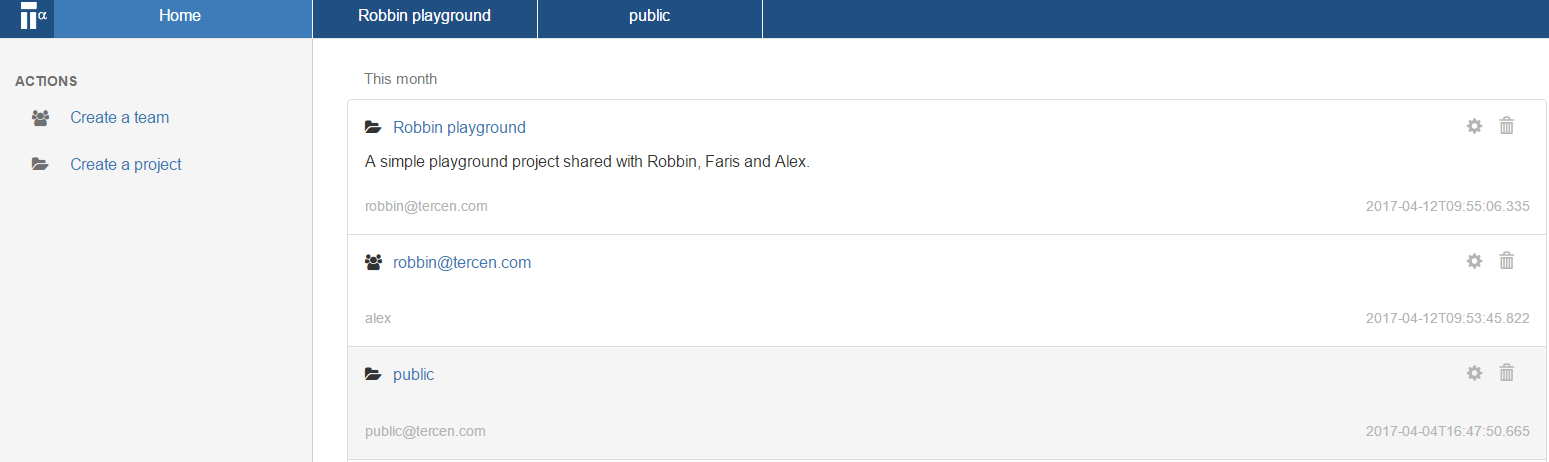
\includegraphics{images/project_home.png}
\caption{}
\end{figure}

\subsubsection{\texorpdfstring{Click on \textbf{Create a data
set}}{Click on Create a data set}}\label{click-on-create-a-data-set}

A dialog window opens which allows you to select the data file.

\begin{figure}[htbp]
\centering
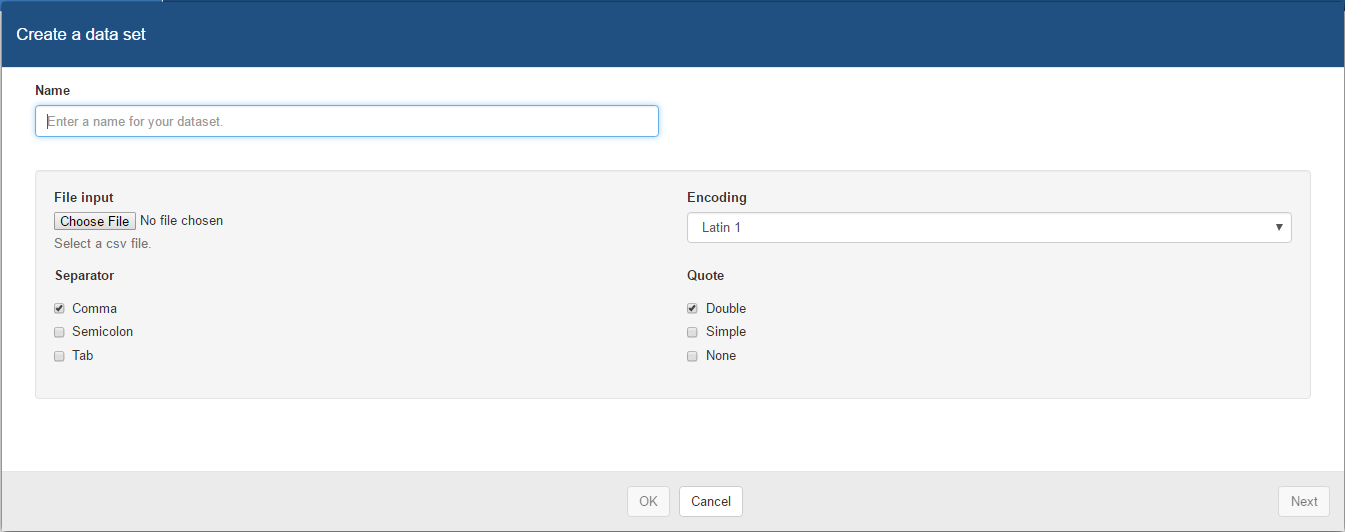
\includegraphics{images/create_dataset.png}
\caption{}
\end{figure}

\subsubsection{\texorpdfstring{Click on the \textbf{Choose File} button
and select your file (i.e
\texttt{crabs\_longformat.csv}).}{Click on the Choose File button and select your file (i.e crabs\_longformat.csv).}}\label{click-on-the-choose-file-button-and-select-your-file-i.e-crabs_longformat.csv.}

Please make sure to select the separator, the encoding and the quote
format.

Selecting the separator requires you to select one of three options:

\begin{itemize}
\tightlist
\item
  Comma (default)
\item
  Semicolon
\item
  Tab
\end{itemize}

Please select \textbf{Comma} for this dataset.

Selecting the encoding requires you to select one of two options:

\begin{itemize}
\tightlist
\item
  Latin 1 (default)
\item
  UTF 8
\end{itemize}

Leave the default.

Selecting the quote requires you to select one of three options:

\begin{itemize}
\tightlist
\item
  Double (Default)
\item
  Simple
\item
  None
\end{itemize}

Leave the default..

\subsubsection{\texorpdfstring{Click
\textbf{Next}}{Click Next}}\label{click-next}

You see what column headers were detected and their associated type.

\subsubsection{\texorpdfstring{Click
\textbf{OK}}{Click OK}}\label{click-ok}

You will now see the new data set in the \emph{project page}.

\section{\texorpdfstring{Creating a
\emph{workflow}}{Creating a workflow}}\label{creating-a-workflow}

\subsubsection{\texorpdfstring{Go to the \emph{project
page}}{Go to the project page}}\label{go-to-the-project-page}

\begin{figure}[htbp]
\centering
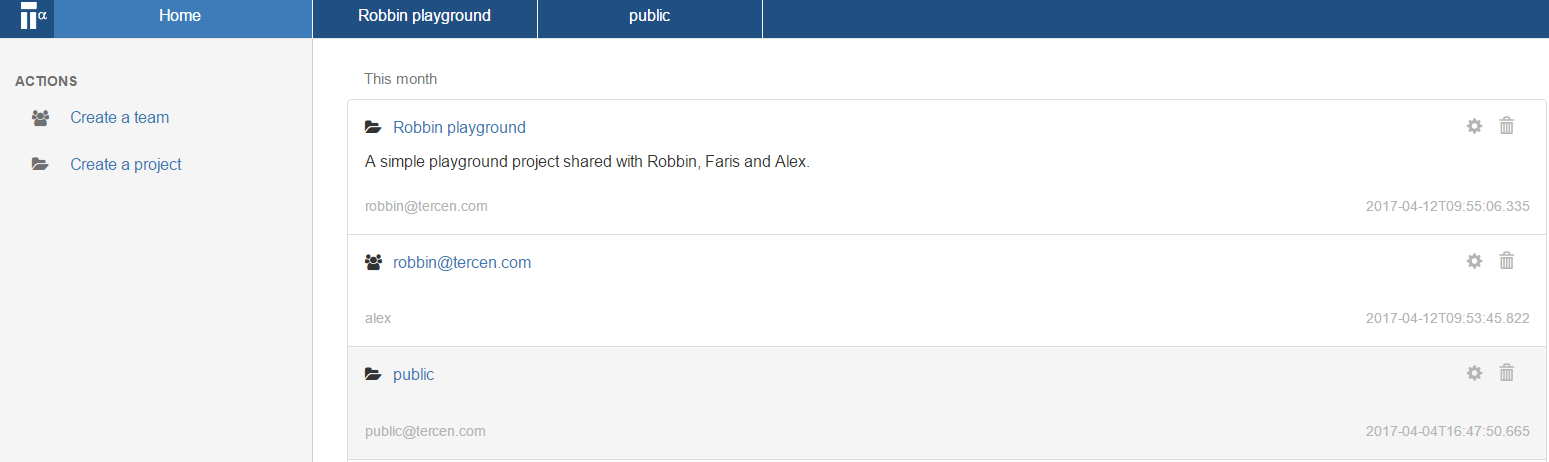
\includegraphics{images/project_home.png}
\caption{}
\end{figure}

\subsubsection{\texorpdfstring{Click on \textbf{Create a
workflow}}{Click on Create a workflow}}\label{click-on-create-a-workflow}

A dialog window opens which allows you to select the data file.

\begin{figure}[htbp]
\centering
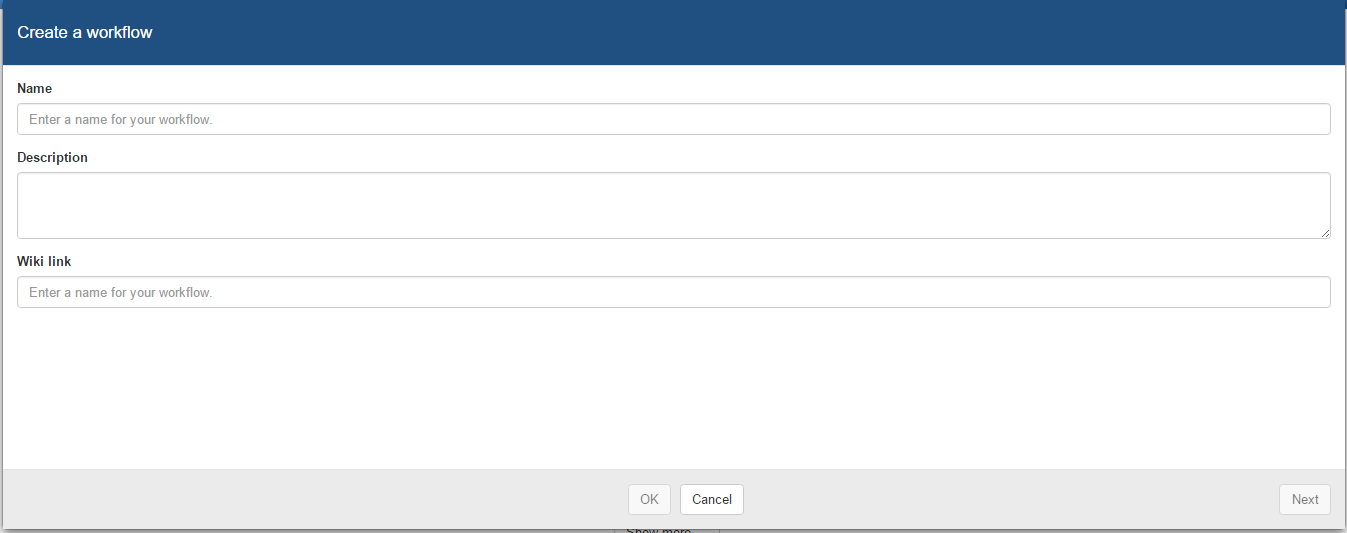
\includegraphics{images/create_workflow.png}
\caption{}
\end{figure}

\subsubsection{\texorpdfstring{Please fill in the \textbf{Name} with the
name
\texttt{crab\ workflow}}{Please fill in the Name with the name crab workflow}}\label{please-fill-in-the-name-with-the-name-crab-workflow}

The following information is possible: * Name (Mandatory) * Description
(Optional) * Wiki Link (Optional)

\subsubsection{\texorpdfstring{Click \textbf{Next} and then click
\textbf{OK}}{Click Next and then click OK}}\label{click-next-and-then-click-ok}

You will now have an empty \emph{workflow page} titled
\texttt{Crab\ workflow} you gave it.

\subsubsection{\texorpdfstring{Right click in the \emph{workflow page}
and select \textbf{Add
step}}{Right click in the workflow page and select Add step}}\label{right-click-in-the-workflow-page-and-select-add-step}

\subsubsection{\texorpdfstring{Select \textbf{Table} and click
\textbf{OK}}{Select Table and click OK}}\label{select-table-and-click-ok}

A new step named Table should appear on your \emph{worklow page}.

\subsubsection{\texorpdfstring{Right click on the Table step and select
\textbf{Run}}{Right click on the Table step and select Run}}\label{right-click-on-the-table-step-and-select-run}

A window appear allowing you to select the data sets which are
available. Select the crab data set you have uploaded.

\subsubsection{\texorpdfstring{Select data set and click
\textbf{OK}}{Select data set and click OK}}\label{select-data-set-and-click-ok}

The Table step should now be green.

You have now successfully imported you data sets into the workflow.

\section{Defining a view}\label{defining-a-view}

Once you have imported your data into the workflow now you can configure
a \textbf{projection}.

\subsubsection{\texorpdfstring{Right click on the Table step and select
\textbf{Add
step}}{Right click on the Table step and select Add step}}\label{right-click-on-the-table-step-and-select-add-step}

\subsubsection{\texorpdfstring{Select \textbf{Data step} and click
\textbf{OK}.}{Select Data step and click OK.}}\label{select-data-step-and-click-ok.}

Your workflow should look like:
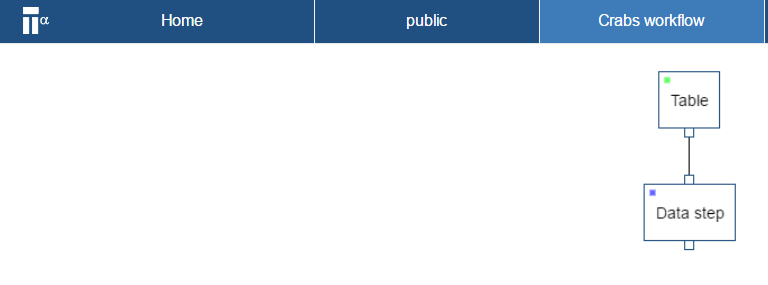
\includegraphics{images/demo_table_data.png}

\subsubsection{Double click on the data
step}\label{double-click-on-the-data-step}

A \emph{projection page} opens

\begin{figure}[htbp]
\centering
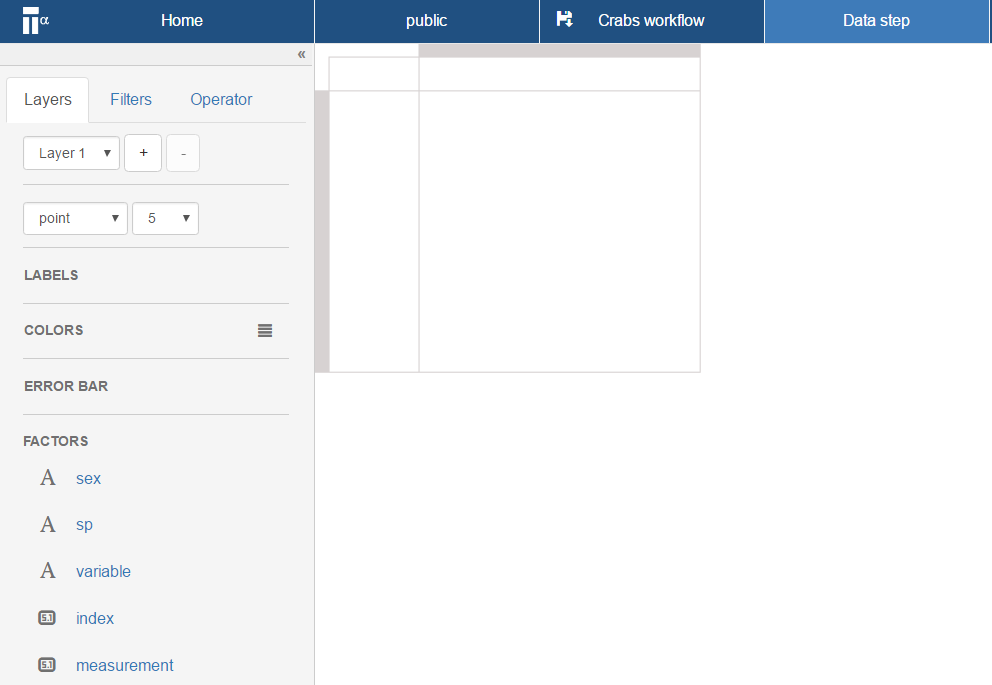
\includegraphics{images/projection.png}
\caption{}
\end{figure}

The \emph{projection} page is composed of different zones. The main
zones are highlighted in green below:

\begin{figure}[htbp]
\centering
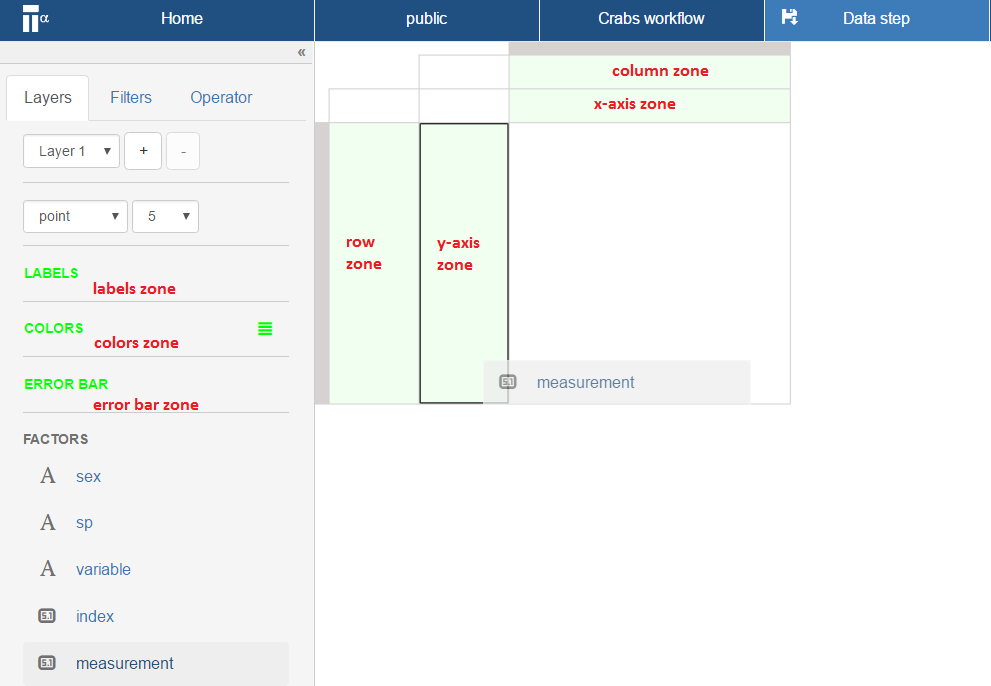
\includegraphics{images/projection_zones.png}
\caption{}
\end{figure}

You can create any projection by dragging-n-dropping of items in the
\emph{factors} list to the different \emph{zones} (indicated by the
color green) of the \emph{projection page}. There are four \emph{zones}
on the right and three on the left.

On the right are:

\begin{itemize}
\tightlist
\item
  \emph{y-axis zone}
\item
  \emph{x-axis zone}
\item
  \emph{column zone}
\item
  \emph{row zone}
\end{itemize}

on the left are:

\begin{itemize}
\tightlist
\item
  \emph{label zone}
\item
  \emph{colors zone}
\item
  \emph{error bar zone}
\end{itemize}

\subsubsection{\texorpdfstring{Drag-n-drop the \texttt{measurement}
factor to the y-axis
zone}{Drag-n-drop the measurement factor to the y-axis zone}}\label{drag-n-drop-the-measurement-factor-to-the-y-axis-zone}

\subsubsection{\texorpdfstring{Drag-n-drop the \texttt{variable} factor
to the row
zone}{Drag-n-drop the variable factor to the row zone}}\label{drag-n-drop-the-variable-factor-to-the-row-zone}

\subsubsection{\texorpdfstring{Drag-n-drop the \texttt{index} and
\texttt{sp} and \texttt{sex} factor to the column
zone}{Drag-n-drop the index and sp and sex factor to the column zone}}\label{drag-n-drop-the-index-and-sp-and-sex-factor-to-the-column-zone}

\begin{figure}[htbp]
\centering
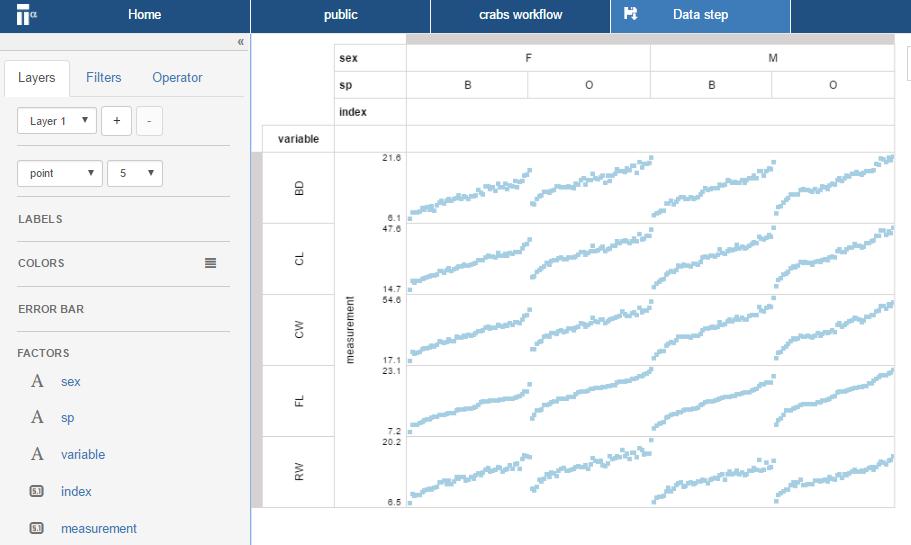
\includegraphics{images/projection_measurement.png}
\caption{}
\end{figure}

The image should look like the one above. Notice, the variable are the
row and the observations are the columns. \#\#\#\# Drag-n-drop the
\texttt{measurement} to colors zone

\subsubsection{\texorpdfstring{Select \texttt{heatmap} in the drop down
menu where it currently says
\texttt{point}}{Select heatmap in the drop down menu where it currently says point}}\label{select-heatmap-in-the-drop-down-menu-where-it-currently-says-point}

The projection window should now show the following:

\begin{figure}[htbp]
\centering
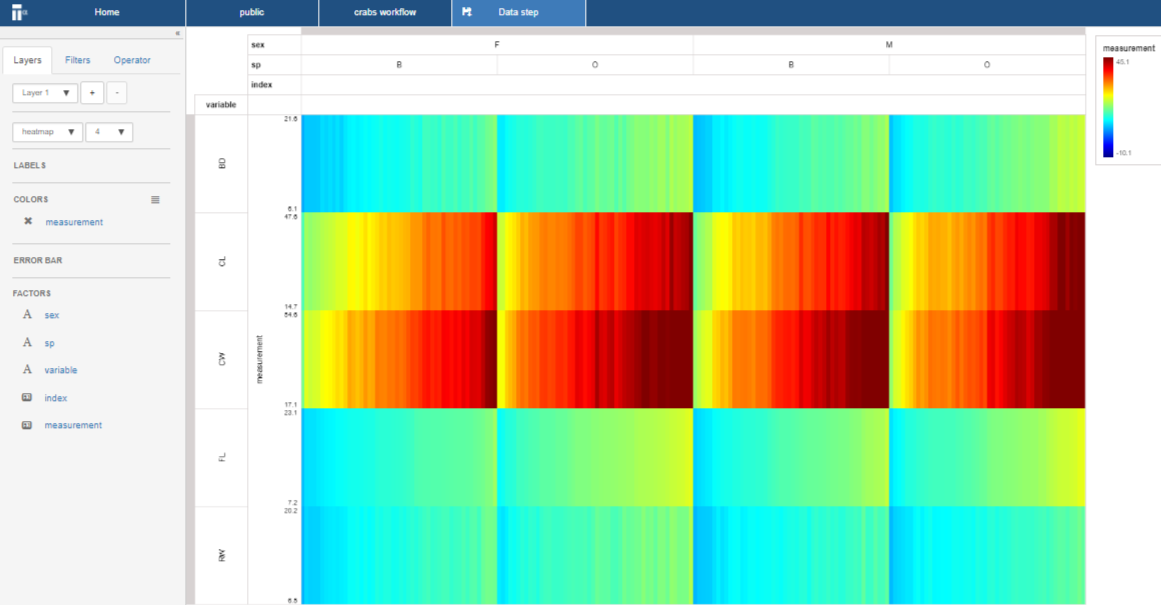
\includegraphics{images/projection_heatmap_crabs.png}
\caption{}
\end{figure}

\section{Computing}\label{computing}

The projection you created in the previous section can also be used by a
computation (i.e. \emph{operator}). This is due to the \emph{What you
see is what you compute} paradigm. The following steps outlines how to
add an \emph{operator}.

\subsubsection{\texorpdfstring{Click on the \textbf{Operator}
tab}{Click on the Operator tab}}\label{click-on-the-operator-tab}

\subsubsection{\texorpdfstring{Go to the \textbf{Public tab} and select
the \texttt{PCA} operator, click
\textbf{OK}}{Go to the Public tab and select the PCA operator, click OK}}\label{go-to-the-public-tab-and-select-the-pca-operator-click-ok}

\subsubsection{Click on the save icon of the Data step page
bar}\label{click-on-the-save-icon-of-the-data-step-page-bar}

The save icon (see red circle in figure below) will dissappear once it
is saved 
\includegraphics{images/save_data_step.png}

\subsubsection{Go to the workflow page}\label{go-to-the-workflow-page}

\subsubsection{\texorpdfstring{Right click on the data step and select
\textbf{Run}}{Right click on the data step and select Run}}\label{right-click-on-the-data-step-and-select-run}

The the data step status color will now go from blue to red (i.e in
progress). Wait until the status goes to green (i.e completed).

\section{Visualizing the result}\label{visualizing-the-result}

\subsubsection{\texorpdfstring{Click on the data step and select
\textbf{Add
step}}{Click on the data step and select Add step}}\label{click-on-the-data-step-and-select-add-step}

\subsubsection{\texorpdfstring{Choose a \textbf{Data step} and click
\textbf{OK}}{Choose a Data step and click OK}}\label{choose-a-data-step-and-click-ok}

\subsubsection{Open the newly created data
step}\label{open-the-newly-created-data-step}

A new projection page opens. This projection page should be familiar as
you have seen this before in the previous steps of the this guide.
However you will notice there are additional factors in the factor list,
namely PC1, PC2, etc..

\subsubsection{\texorpdfstring{Drag-n-drop the \texttt{PC2} factor to
the \emph{x-axis
zone}}{Drag-n-drop the PC2 factor to the x-axis zone}}\label{drag-n-drop-the-pc2-factor-to-the-x-axis-zone}

\subsubsection{\texorpdfstring{Drag-n-drop the \texttt{PC3} factor to
the \emph{y-axis
zone}}{Drag-n-drop the PC3 factor to the y-axis zone}}\label{drag-n-drop-the-pc3-factor-to-the-y-axis-zone}

\subsubsection{\texorpdfstring{Drag-n-drop the \texttt{sex} and
\texttt{species} factor to the \emph{colors
zone}}{Drag-n-drop the sex and species factor to the colors zone}}\label{drag-n-drop-the-sex-and-species-factor-to-the-colors-zone}

\begin{figure}[htbp]
\centering
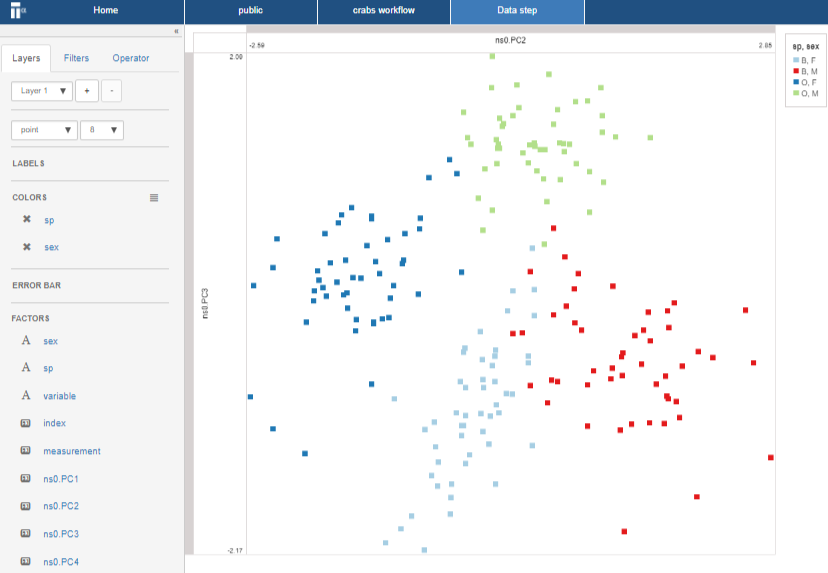
\includegraphics{images/projection_pca.png}
\caption{}
\end{figure}

\section{Visualizing a pairwise}\label{visualizing-a-pairwise}

\subsubsection{\texorpdfstring{Click on the first data step and select
\textbf{Add
step}}{Click on the first data step and select Add step}}\label{click-on-the-first-data-step-and-select-add-step}

\subsubsection{\texorpdfstring{Choose a \textbf{Data step} and click
\textbf{OK}}{Choose a Data step and click OK}}\label{choose-a-data-step-and-click-ok-1}

This will create a second data step (see workflow screen shot below)

\subsubsection{Open the newly created data
step}\label{open-the-newly-created-data-step-1}

A new projection page opens. We will now create a pairwise projection of
the \texttt{variable}.

\subsubsection{\texorpdfstring{Drag-n-drop the \texttt{variable} factor
to the \emph{column
zone}}{Drag-n-drop the variable factor to the column zone}}\label{drag-n-drop-the-variable-factor-to-the-column-zone}

\subsubsection{\texorpdfstring{Drag-n-drop the \texttt{variable} factor
to the \emph{row
zone}}{Drag-n-drop the variable factor to the row zone}}\label{drag-n-drop-the-variable-factor-to-the-row-zone-1}

\subsubsection{\texorpdfstring{Drag-n-drop the \texttt{index} and
\texttt{species} factor to the \emph{label
zone}}{Drag-n-drop the index and species factor to the label zone}}\label{drag-n-drop-the-index-and-species-factor-to-the-label-zone}

\begin{figure}[htbp]
\centering
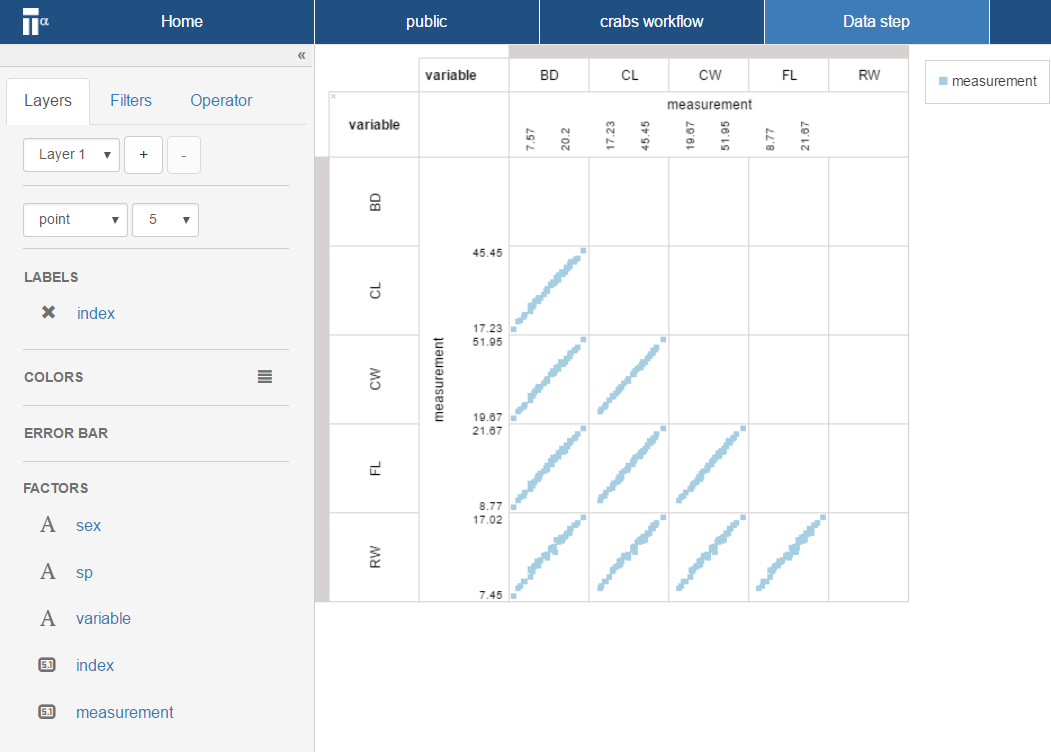
\includegraphics{images/projection_pairwise.png}
\caption{}
\end{figure}

This is the first pairwise projection, however these projection can be
further developed into multi-group pariwise.

\subsubsection{\texorpdfstring{Drag-n-drop the \texttt{sex} factor to
the \emph{column
zone}}{Drag-n-drop the sex factor to the column zone}}\label{drag-n-drop-the-sex-factor-to-the-column-zone}

\subsubsection{\texorpdfstring{Drag-n-drop the \texttt{sp} factor to the
\emph{color
zone}}{Drag-n-drop the sp factor to the color zone}}\label{drag-n-drop-the-sp-factor-to-the-color-zone}

\begin{figure}[htbp]
\centering
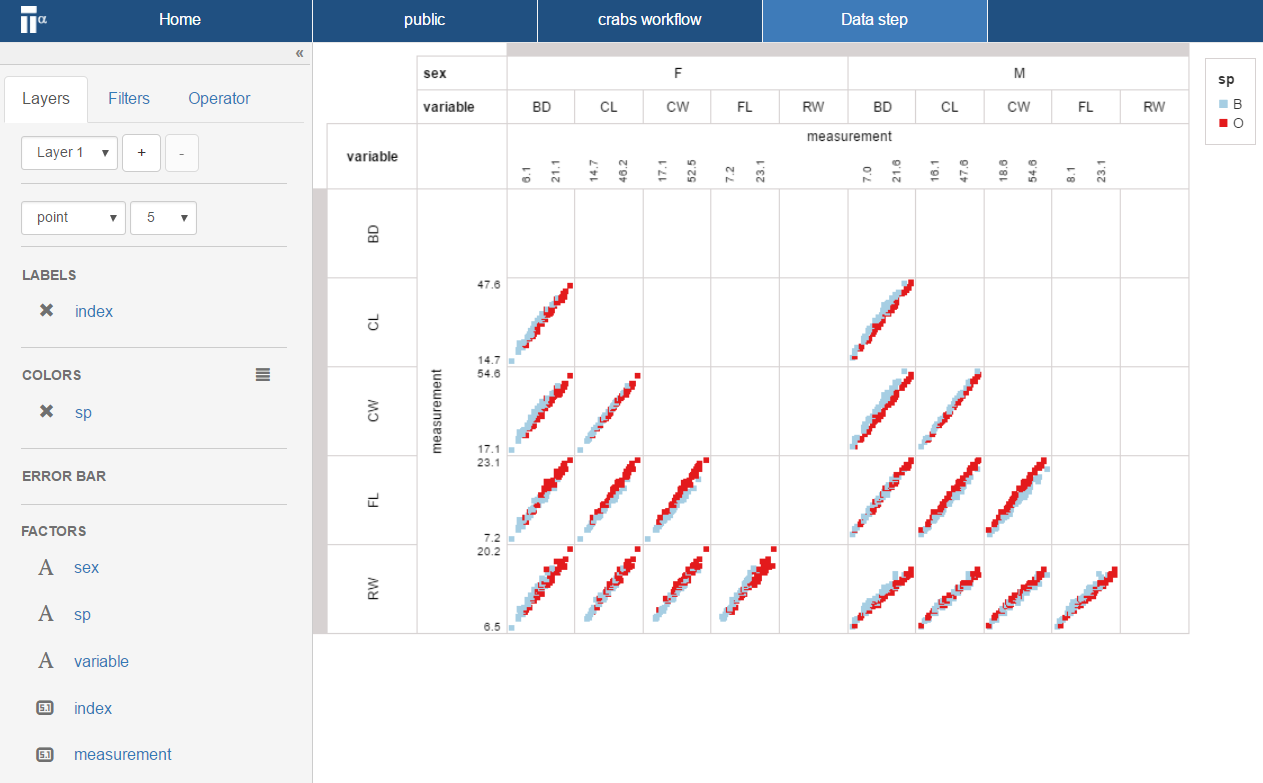
\includegraphics{images/projection_pairwise_2.png}
\caption{}
\end{figure}

You have now completed the multi-group pairwise. This view is a powerful
projection.

Your workflow should look like the following:

\begin{figure}[htbp]
\centering
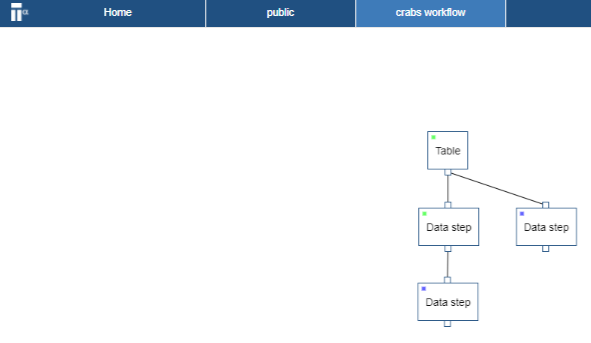
\includegraphics{images/workflow_crabs.png}
\caption{}
\end{figure}

\section{Sharing the result}\label{sharing-the-result}

You will notice the each \emph{data step} (and hence visual) has its own
unique URL and each \emph{workflow} has its own unique URL.

\url{https://tercen.com/core/\#w/fa51aae551f7c3d14727ab5fd9b65433}

This URL is for the crabs workflow found in the `'public'' project

\subsubsection{Copy the url of the view with the multi-group
plot}\label{copy-the-url-of-the-view-with-the-multi-group-plot}

You can send this URL to another person by email or via a chat session.

\url{https://tercen.com/core/\#ds/fa51aae551f7c3d14727ab5fd9b65433/2efff9f0-0f80-11e7-8de2-9fe5ab3cbd24}

This URL is for the multi-group pairwise found in the workflow in the
`'public'' project

\chapter{Operators}\label{operators}

Some \emph{significant} operators are demonstrated in this chapter.

\section{Operator one}\label{operator-one}

\section{Operator two}\label{operator-two}

\chapter{Applications}\label{applications}

Some \emph{significant} applications are demonstrated in this chapter.

\section{Example one}\label{example-one}

\section{Example two}\label{example-two}

\chapter{Applications}\label{applications-1}

Some \emph{significant} applications are demonstrated in this chapter.

\section{Example one}\label{example-one-1}

\section{Example two}\label{example-two-1}


\end{document}
